% ============================================================
% ropfec: An open, reproducible implementation of
% reaction-order-polyhedron-constrained flux exponent control,
% with an honest analysis of when binding structure helps.
%
% Preprint source. Engine: XeTeX (tectonic) or pdfLaTeX.
% Build:  tectonic ropfec.tex   (runs bibtex automatically)
% ============================================================
\documentclass[11pt]{article}

\usepackage{geometry}
\geometry{margin=1in}
\usepackage{amsmath,amssymb}
\usepackage{graphicx}
\usepackage{booktabs}
\usepackage{algorithm}
\usepackage{algpseudocode}
\usepackage{tikz}
\usetikzlibrary{arrows.meta,positioning,fit,backgrounds,calc}
\usepackage{xcolor}
\usepackage[numbers,sort&compress]{natbib}
\usepackage{hyperref}
\hypersetup{
  colorlinks=true, linkcolor=blue!55!black, citecolor=blue!55!black,
  urlcolor=blue!55!black, breaklinks=true
}

\newcommand{\rop}{\mathrm{ROP}}
\newcommand{\real}{\mathbb{R}}

\title{\textbf{An open, reproducible implementation of\\
reaction-order-polyhedron--constrained flux exponent control,\\
and an honest analysis of when binding structure helps}}

\author{Lei Zhou\thanks{Zhejiang A\&F University, Hang\-zhou, China.
Correspondence: \href{mailto:exergyleizhou@gmail.com}{exergyleizhou@gmail.com};
ORCID 0009-0000-9073-1349.}}

\date{\today}

\begin{document}
\maketitle

\begin{abstract}
\noindent
Xiao, Li and Doyle's \emph{flux exponent control} (FEC) and its underlying
\emph{reaction order polyhedron} (ROP) propose that metabolic dynamics can be
predicted and controlled from network structure: the reaction-order exponents of
a power-law kinetic model are constrained, by binding stoichiometry, to a
polyhedron, and dynamic regulation is the solution of an optimal-control problem
over that polyhedron. The framework is attractive because it avoids full
kinetic-parameter identification, but it has existed as theory and an MPC concept
without an open, tested implementation. We contribute three things.
\textbf{(i)~A reproducible reference implementation}, \texttt{ropfec}: ROP
H-representation construction, ROP-constrained FEC as a CasADi/IPOPT
optimal-control problem, interval/robust and multicellular extensions, and a
modular closed-loop integration with reference component implementations; 44
automated tests; one-command reproduction. On an in-silico glycolysis benchmark,
enforcing the binding-derived ROP reduces trajectory prediction error
$\sim\!3.2\times$ versus an out-of-polyhedron exponent, and the FEC solver tracks
a target flux to within $0.5\%$ of ground truth. \textbf{(ii)~A clarifying
connection}: FEC's controlled exponents are exactly the elasticity coefficients
of metabolic control analysis (MCA), placing FEC within a classical formalism
rather than treating it as an ad hoc parameterization. We also provide two
published glycolytic-oscillator models (Sel'kov; Wolf--Heinrich) as validated
re-implementations and reusable testbeds. \textbf{(iii)~An honest negative
result}: we test whether the binding-derived ROP, used as a structural prior,
improves \emph{data-driven} estimation of reaction orders, and find it does not
--- when rate data are informative the ROP is inactive, and when data are scarce
it tightens the feasible set no more than a count-matched random set. The value
of ROP/FEC is therefore as a structural \emph{modelling and control} framework,
not as a statistical regulariser for identification. We are explicit about scope:
all results are in-silico with reference components and no wet-lab data. The
software is intended as a reproducible reference and an honest map of where the
framework does and does not add value.
\end{abstract}

\noindent\textbf{Keywords:} flux exponent control; reaction order polyhedron;
metabolic control analysis; optimal control; chemical reaction networks;
reproducible software; uncertainty.

\tableofcontents

% =====================================================================
\section{Introduction}
% =====================================================================

Predicting and controlling the \emph{dynamics} of metabolism from network
structure sits between two established extremes. Flux balance analysis (FBA)
predicts steady-state fluxes from stoichiometry and an optimality principle with
no kinetic parameters, but is static~\citep{orth2010fba,varma1994stoichiometric}.
Mechanistic kinetic models capture dynamics but require many poorly identifiable
parameters~\citep{saa2017kinetic}. A range of approximate frameworks --- dynamic
FBA~\citep{mahadevan2002dfba}, lin-log kinetics~\citep{hatzimanikatis1997loglinear,
visser2003linlog}, and ensemble methods~\citep{miskovic2010oracle,smallbone2007bridging}
--- occupy the middle ground.

Xiao, Li and Doyle proposed another middle-ground
approach~\citep{xiao2023fec,xiao2022thesis}. In a power-law kinetic description
the \emph{reaction orders} (the exponents on concentrations) are not free:
binding stoichiometry constrains them to a polyhedron, the \emph{reaction order
polyhedron} (ROP), whose continuous analogue is the log-derivative of the rate.
\emph{Flux exponent control} (FEC) posits that cells regulate flux exponents and
that dynamic regulation solves an optimal-control problem over the ROP, tractable
by model predictive control (MPC)~\citep{rawlings2017mpc}. Because the admissible
exponents come from structure, FEC predicts dynamics --- glycolytic oscillations
being the motivating example --- without full parameter identification.

To be used and built upon, this framework needs an open, tested implementation,
and an honest account of where its structural prior actually helps. We provide
both, while being deliberately conservative about novelty: the ideas (ROP, FEC,
the log-derivative structure) are Xiao et al.'s. Our contributions are:

\begin{itemize}
\item[\textbf{C1}] \textbf{A reproducible reference implementation}
(\S\ref{sec:methods}) of ROP construction and ROP-constrained FEC
(CasADi/IPOPT~\citep{andersson2019casadi,wachter2006ipopt}), with interval/robust
and multicellular extensions and a modular closed-loop integration, validated
in-silico (\S\ref{sec:results}).
\item[\textbf{C2}] \textbf{The MCA-elasticity identity} (\S\ref{sec:mca}): FEC's
controlled exponents are metabolic-control-analysis elasticities, a connection
that grounds the framework and that, to our knowledge, the FEC literature does
not make explicit.
\item[\textbf{C3}] \textbf{An honest negative result} (\S\ref{sec:negative}):
the binding-derived ROP does not improve data-driven order estimation, which
sharpens \emph{where} the framework adds value (control, not identification).
\end{itemize}

% =====================================================================
\section{Background}\label{sec:background}
% =====================================================================

We restate the constructs we implement, following~\citet{xiao2023fec} and
\citet{xiao2022thesis}, to fix notation.

\paragraph{Power-law kinetics on a CRN.} For a chemical reaction network with $n$
species, concentrations $x\in\real^n_{\ge 0}$, $m$ reactions with stoichiometric
matrix $N$, and power-law rates~\citep{feinberg2019crnt,alon2019systems},
\begin{equation}
v_r(x) = k_r \prod_{i=1}^{n} x_i^{\alpha_{r,i}}, \qquad \dot{x} = N\,v(x,\alpha).
\label{eq:powerlaw}
\end{equation}

\paragraph{Reaction order polyhedron (ROP).} Binding stoichiometry and
physical bounds constrain $\alpha$ to a polyhedron~\citep{xiao2022thesis},
\begin{equation}
\rop \triangleq \bigl\{ \alpha \;\big|\; A\,\alpha \le b,\ \alpha \ge 0 \bigr\},
\qquad
L_{r,i}(\alpha) \triangleq \frac{\partial \log v_r}{\partial \log x_i} = \alpha_{r,i}.
\label{eq:rop}
\end{equation}

\paragraph{Flux exponent control (FEC).} Dynamic regulation is cast as control of
the exponents subject to the ROP~\citep{xiao2023fec}:
\begin{align}
\min_{\alpha(\cdot)} & \int_0^T \ell\bigl(x(t),f(t),\alpha(t)\bigr)\,dt
\quad \text{s.t.} \quad \dot{x} = N v(x,\alpha),\ \ \alpha(t)\in\rop,\ \ f = v(x,\alpha).
\label{eq:fec}
\end{align}

\subsection{Reaction orders are metabolic-control-analysis elasticities}\label{sec:mca}

A connection worth making explicit: the log-derivative~\eqref{eq:rop} that FEC
controls \emph{is} the elasticity coefficient of metabolic control analysis (MCA).
MCA defines the elasticity of a rate $v$ to a metabolite $x$ as the scaled
derivative $\varepsilon^{v}_{x} = (\partial v/\partial x)(x/v) = \partial \ln
v/\partial \ln x$~\citep{kacser1973control,heinrich1974linear,fell1997understanding}.
Comparing with~\eqref{eq:rop}, the FEC exponent $\alpha_{r,i}$ is exactly the
elasticity $\varepsilon^{v_r}_{x_i}$. FEC thus inherits MCA's local-sensitivity
interpretation --- each exponent is the fractional change in flux per fractional
change in a metabolite at the operating point --- and the assumption that the
exponent is approximately constant over a regime is the standard local
(lin-log / power-law) approximation~\citep{hatzimanikatis1997loglinear,visser2003linlog}.
We are careful with MCA vocabulary: $\alpha$ is an \emph{elasticity} (a local,
single-reaction property), not a systemic flux-control coefficient. This identity
is not new to MCA; making it the basis of FEC's control variable is the small
clarifying point.

% =====================================================================
\section{Methods: the \texttt{ropfec} implementation}\label{sec:methods}
% =====================================================================

\texttt{ropfec} is a small Python package (NumPy/SciPy/CasADi) around the
constructs of \S\ref{sec:background}; Figure~\ref{fig:arch} shows the closed-loop
architecture.

\begin{figure}[t]
\centering
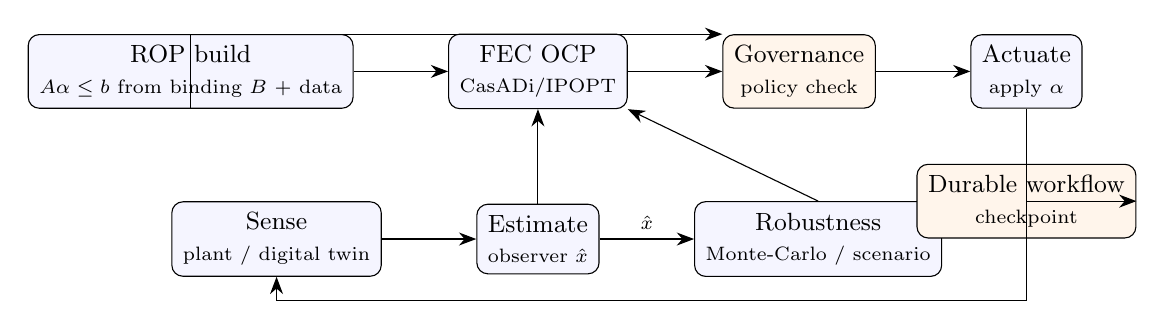
\begin{tikzpicture}[
  font=\small,
  box/.style={draw, rounded corners, align=center, minimum height=8mm, inner sep=4pt, fill=blue!4},
  gov/.style={draw, rounded corners, align=center, minimum height=8mm, inner sep=4pt, fill=orange!8},
  >={Stealth[length=2.2mm]}, node distance=7mm and 12mm]
\node[box] (rop) {ROP build\\ \scriptsize $A\alpha\le b$ from binding $B$ + data};
\node[box, right=of rop] (fec) {FEC OCP\\ \scriptsize CasADi/IPOPT};
\node[gov, right=of fec] (opa) {Governance\\ \scriptsize policy check};
\node[box, right=of opa] (act) {Actuate\\ \scriptsize apply $\alpha$};
\node[box, below=12mm of fec] (est) {Estimate\\ \scriptsize observer $\hat{x}$};
\node[box, left=of est] (sense) {Sense\\ \scriptsize plant / digital twin};
\node[box, right=of est] (mc) {Robustness\\ \scriptsize Monte-Carlo / scenario};
\node[gov, below=7mm of act, align=center] (wf) {Durable workflow\\ \scriptsize checkpoint};
\draw[->] (rop) -- (fec);
\draw[->] (fec) -- (opa);
\draw[->] (opa) -- (act);
\draw[->] (act) |- (wf.east);
\draw[->] (sense) -- (est);
\draw[->] (est) -- node[above,font=\scriptsize]{$\hat{x}$} (mc);
\draw[->] (est.north) -- (fec.south);
\draw[->] (mc.north) -- (fec.south east);
\draw[->] (act.south) |- ([yshift=-3mm]sense.south) -| (sense.south);
\draw[->] (rop.south) |- (opa.north west);
\end{tikzpicture}
\caption{Closed-loop architecture implemented by \texttt{ropfec}. The ROP is
built once from binding stoichiometry and data and supplies hard constraints to
the FEC optimal-control problem and the governance check. The estimation,
robustness, governance and workflow blocks are reference implementations
(\S\ref{sec:integration}).}
\label{fig:arch}
\end{figure}

\subsection{ROP construction and FEC solver}\label{sec:fec}

\texttt{rop\_polyhedron.py} builds the H-representation~\eqref{eq:rop} from
binding stoichiometry (optionally augmented with data-driven bounds from
log-linear regression of measured rates against log-concentrations) and exposes
feasibility, Euclidean projection $\Pi_{\rop}$, and the log-derivative matrix.
\texttt{fec\_solver.py} transcribes problem~\eqref{eq:fec} into an NLP: the
dynamics are integrated over a horizon, the ROP membership is imposed as the
linear constraint $A\alpha\le b$ directly in the solver, and the objective tracks
a reference flux. The NLP is built with CasADi~\citep{andersson2019casadi} and
solved with IPOPT~\citep{wachter2006ipopt}; a projection fallback is used when
CasADi/IPOPT are unavailable.

\subsection{Interval/robust and multicellular extensions}\label{sec:robust}

\texttt{robust\_extension.py} implements an interval ROP and a sampled
scenario (min--max) robust FEC over a digital-twin uncertainty set, using
standard robust/scenario MPC machinery~\citep{kothare1996robust,scokaert1998minmax,
mayne2005tube,calafiore2006scenario,campi2008exact,bertsimas2011robust};
\texttt{multicell\_agent.py} scales the loop to a consortium coupled by a quorum
signal with a population-level resource policy.

\subsection{Data-driven order-uncertainty sets}\label{sec:orderuq}

\texttt{order\_uncertainty.py} builds, from noisy $(x,v)$ data, a bounded-error
set over the orders: under $|\log v_i - (\alpha\!\cdot\!\log x_i + \log k)| \le
\epsilon$ the data-consistent parameters form a polytope $A_{\mathrm{data}}\theta
\le b_{\mathrm{data}}$ with $\theta=[\alpha,\log k]$. We can intersect this with
the binding-derived ROP, take the axis-aligned bounding box, and measure the
worst-case spread of any linear functional (e.g.\ the predicted log-flux
$\alpha\!\cdot\!\log x^\star + \log k$). This machinery supports the analysis in
\S\ref{sec:negative}.

\subsection{Closed-loop integration and its honest scope}\label{sec:integration}

The blocks around the FEC solver in Figure~\ref{fig:arch} (estimation,
Monte-Carlo robustness, governance, durable workflow) are accessed through narrow
interfaces, with \emph{reference implementations} shipped so the loop runs and
tests end to end. \textbf{The results in this paper use these reference
components, not a production platform}; the interface design lets each be replaced
without changing the FEC core.

\subsection{Case-study models}\label{sec:casestudy}

To exercise the implementation beyond a single toy, we provide validated
re-implementations of two published glycolytic-oscillator models: the
two-variable Sel'kov model~\citep{selkov1968} and the single-cell core of the
Wolf--Heinrich yeast model~\citep{wolf2000}. Both are pure NumPy/SciPy and ship
with tests asserting the known limit-cycle behaviour; the larger Chassagnole
\emph{E.\,coli} model~\citep{chassagnole2002} is noted as a scalability target
for future work.

\subsection{Software, tests and reproducibility}\label{sec:repro}

\texttt{ropfec} runs on Python~3.9 with NumPy/SciPy/CasADi/Matplotlib; randomised
components use fixed seeds. A suite of 44 automated tests (33 engine + 11
case-study) covers ROP construction/projection, the FEC solver (CasADi path and
fallback), the robust and multicellular extensions, the order-uncertainty
machinery, the FBA/MM benchmark, numerical stability, the end-to-end loop
invariants, and the case-study oscillations. A single command reruns the tests
and regenerates every figure and number reported below.

% =====================================================================
\section{Results}\label{sec:results}
% =====================================================================

\subsection{The ROP constraint matters for control (in-silico toy)}\label{sec:toy}

On a glycolysis-like toy CRN ($n=3$, $m=4$, the Xiao running example), with a
$6$-facet binding-derived ROP, we compare a synthetic ground-truth trajectory
(binding-limited exponents $\alpha_{\text{gt}}=[0.6,0.85,1.7]$) against an
unconstrained exponent whose third component lies outside the polyhedron
($\alpha_2=3.1>2$) and the same exponent projected onto the ROP
(Figure~\ref{fig:toy}). The out-of-polyhedron exponent gives a mean trajectory
error of $9.9\%$; projecting onto the ROP reduces it to $3.1\%$ --- a factor
$\sim\!3.2$ --- purely by respecting structure. The FEC solver, tracking a target
flux, returns $\alpha^\star=[0.6,0.84,1.62]\in\rop$ matching ground truth to
within $0.5\%$. Against in-ROP FBA- and MM-derived exponent policies (50 runs),
the FEC optimal-control policy attains the lowest final-state tracking cost
($1.01$ vs $1.28$ and $1.09$; Table~\ref{tab:fbamm}), and a scenario-robust
policy matches the nominal cost while bounding the worst case. The ground truth
here is synthetic, so these results demonstrate the \emph{mechanism} (respecting
the binding constraint), not empirical accuracy on biological data.

\begin{figure}[t]
\centering
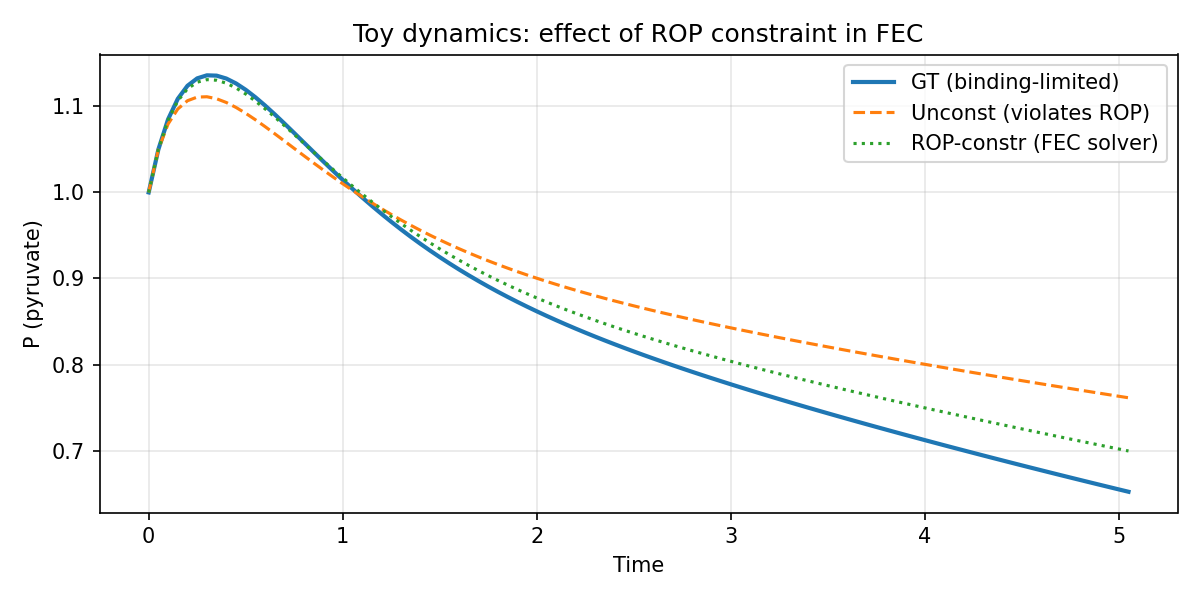
\includegraphics[width=0.72\textwidth]{figures/toy_traj_comparison.png}
\caption{In-silico toy dynamics: pyruvate under the ground-truth exponent, an
unconstrained exponent that violates the ROP, and the FEC/ROP-constrained
exponent. Respecting the binding-derived polyhedron recovers ground-truth
dynamics (mean error $3.1\%$ vs $9.9\%$).}
\label{fig:toy}
\end{figure}

\begin{table}[t]
\centering
\caption{Final-state tracking cost (L2 to target; lower is better) over $50$ runs
on the toy network. All policies are projected into the ROP, so the difference
reflects exponent quality only.}
\label{tab:fbamm}
\begin{tabular}{lcc}
\toprule
Policy & Mean cost & vs.\ FEC \\
\midrule
FBA-derived (in ROP)         & $1.283$ & $1.27\times$ worse \\
MM-derived (in ROP)          & $1.090$ & $1.08\times$ worse \\
\textbf{FEC / ROP (ours)}    & $\mathbf{1.011}$ & --- \\
Robust scenario              & $1.011$ & matches nominal \\
\bottomrule
\end{tabular}
\end{table}

\subsection{Case-study oscillators reproduce known dynamics}\label{sec:caseresults}

The Sel'kov and Wolf--Heinrich re-implementations reproduce the published
qualitative behaviour (Figure~\ref{fig:osc}): Sel'kov settles onto a stable limit
cycle inside its Hopf window and to a fixed point outside it, and the
Wolf--Heinrich single-cell core sustains glycolytic oscillations. These serve as
reusable, tested testbeds for the FEC pipeline beyond the toy network.

\begin{figure}[t]
\centering
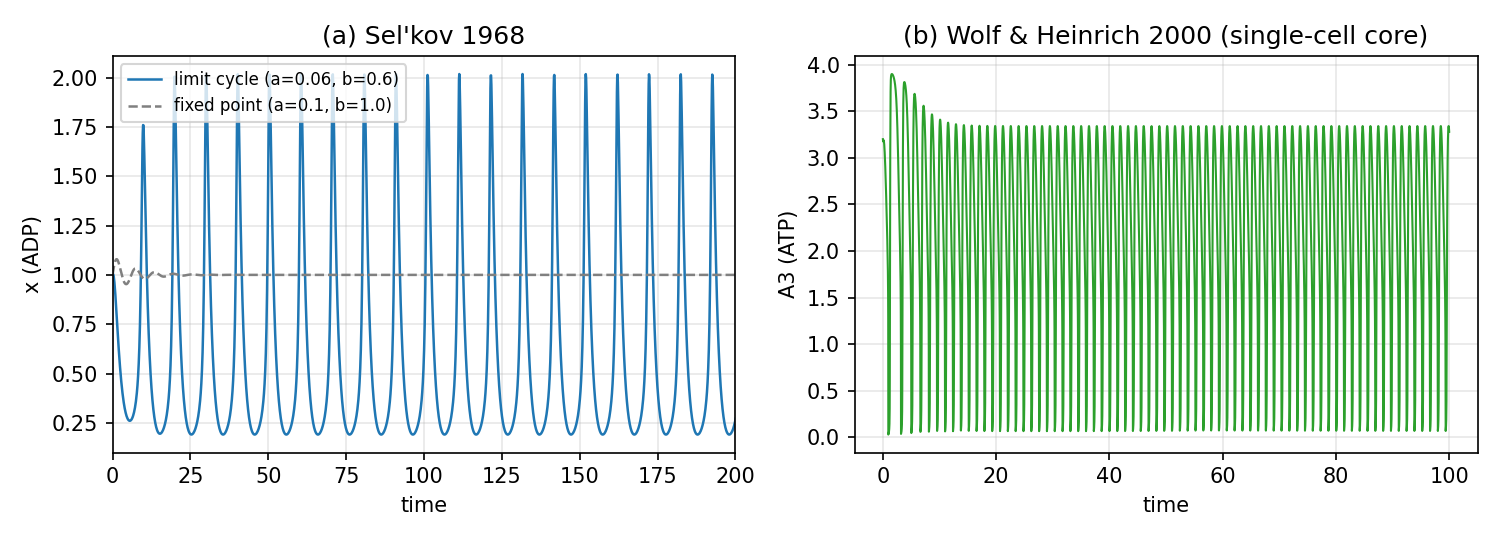
\includegraphics[width=0.95\textwidth]{figures/case_studies_oscillations.png}
\caption{Validated re-implementations of two published glycolytic oscillators:
(a) Sel'kov 1968 (limit cycle vs.\ damped fixed point); (b) Wolf--Heinrich 2000
single-cell core (sustained oscillation of an ATP-like cofactor).}
\label{fig:osc}
\end{figure}

\subsection{A negative result: binding structure does not improve data-driven order estimation}\label{sec:negative}

A natural hope is that the binding-derived ROP, used as a prior, tightens
data-driven estimation of reaction orders. We tested this honestly. From noisy
rate data we built the bounded-error order set (\S\ref{sec:orderuq}) and compared
three feasible sets: the data set alone, the data set intersected with the ROP,
and the data set intersected with a \emph{count-matched random} facet set
calibrated to still contain the true orders (a control for ``more facets'' versus
``the right facets''~\citep{bental1998robust}). We measured the total reaction-order
uncertainty (sum of per-order ranges) in an informative-data regime and a
data-poor regime (Figure~\ref{fig:neg}).

The result is negative. When data are informative, the ROP is \emph{inactive}:
the data set, data$\cap$ROP, and data$\cap$random sets have identical order
uncertainty ($\approx\!0.048$) --- the data already constrain the orders tighter
than the ROP does, and the ROP facets never bind. When data are scarce, the ROP
tightens the set only modestly ($2.80\!\to\!2.34$) and \emph{no more than the
count-matched random set} ($2.42$). Across trials neither beats the other
consistently. We also confirmed on the toy network that, for an informative
sample, the worst-case predicted-flux spread under data$\cap$ROP equals that
under the data alone (the ROP facets are inactive), so the apparent
``tightening versus a box'' is a property of the data's own correlation, not of
the binding mechanism.

\begin{figure}[t]
\centering
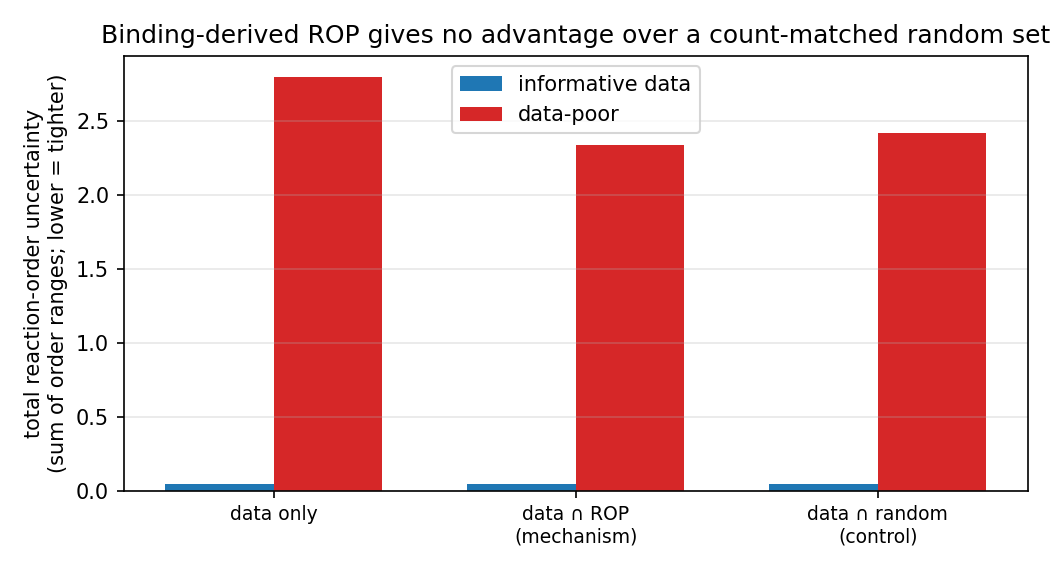
\includegraphics[width=0.72\textwidth]{figures/order_uq_negative.png}
\caption{Honest negative result. Total reaction-order uncertainty for the
data-only set, data$\cap$ROP, and data$\cap$random (count-matched, truth-covering)
sets, in informative and data-poor regimes. The binding-derived ROP confers no
advantage over a random set of equal size: when data are informative it is
inactive; when data are scarce it is no better than chance.}
\label{fig:neg}
\end{figure}

The interpretation is clarifying rather than discouraging: the value of ROP/FEC
is as a structural \emph{modelling and control} framework --- it specifies the
admissible exponent geometry the controller must respect (\S\ref{sec:toy}) --- not
as a statistical regulariser for \emph{identification}. Structure constrains what
the controller may do; it does not, by itself, tell you more about the plant than
the data already do.

\subsection{End-to-end loop integrity}

Running the full loop of Figure~\ref{fig:arch} on the toy network, every
structural invariant holds: the applied exponent is in the ROP at every step, the
published polyhedron matches the constructed one, the observer maintains a
covariance, workflow checkpoints accumulate, governance violations are detected
and counted, and the digital twin replays the FEC trajectory. In the
multicellular setting the resource policy blocks $100\%$ of over-capacity
configurations.

% =====================================================================
\section{Discussion}\label{sec:discussion}
% =====================================================================

\paragraph{What \texttt{ropfec} adds.} Relative to the originating
work~\citep{xiao2023fec,xiao2022thesis} we contribute an open, tested
implementation, a closed-loop integration, robust/multicellular extensions, the
explicit MCA-elasticity identity, and an honest map of where the structural prior
helps. Relative to FBA~\citep{orth2010fba} the framework is dynamic; relative to
full kinetic models it needs only binding-derived order bounds.

\paragraph{Control versus identification.} The two empirical findings cut in
opposite directions and are both honest. The ROP constraint clearly matters for
\emph{control} (\S\ref{sec:toy}): an exponent outside the polyhedron mis-predicts
dynamics, and enforcing the polyhedron recovers them. The same ROP does
\emph{not} help \emph{identification} (\S\ref{sec:negative}): given data, the
binding structure adds nothing a generic constraint of equal size would not. This
distinction --- structure as a control admissibility set, not an estimation prior
--- is, we think, the most useful thing the paper says.

\paragraph{Limitations.} (i)~\emph{In-silico only}: no wet-lab data, no kinetic
parameters identified from experiment; the toy ground truth is synthetic.
(ii)~\emph{Small networks}: validation uses a $3$-species toy plus two small
oscillators; genome-scale conditioning is untested. (iii)~\emph{Reference
components}: the loop's estimation/robustness/governance blocks are reference
implementations, not a deployment. (iv)~The negative result is established on a
binding-derived ROP of modest dimension; we do not claim it for every conceivable
structural prior.

\paragraph{Future work.} Identify a real binding-stoichiometry specification and
rate measurements for a small pathway and test FEC predictions against measured
transients; scale to the Chassagnole network~\citep{chassagnole2002}; and replace
the reference components with production observers and policy engines.

% =====================================================================
\section{Conclusion}
% =====================================================================

We presented \texttt{ropfec}, an open and reproducible implementation of
reaction-order-polyhedron--constrained flux exponent control, with in-silico
validation, the clarifying identity that FEC exponents are MCA elasticities, and
an honest negative result delimiting where the binding-derived structure helps
(control, not identification). The work is offered as a reproducible reference and
an honest account, not an overclaimed method.

% =====================================================================
\section*{Code and data availability}
% =====================================================================

The \texttt{ropfec} source, the 44 tests, and the script that regenerates every
figure and number will be released under an open-source license and archived with
a DOI on Zenodo upon posting. (Repository URL and DOI to be finalised.)

% =====================================================================
\section*{Declarations}
% =====================================================================

\paragraph{Use of AI tools.} Drafting of code and text was assisted by AI tools
(xAI Grok and Anthropic Claude). The author reviewed, verified, and is solely
responsible for all content, including every quantitative claim and citation; all
reported numbers were reproduced by the author from the released code. The AI
tools are not authors.

\paragraph{Competing interests.} The author declares no competing interests.

\paragraph{Funding.} This research received no specific grant from funding
agencies in the public, commercial, or not-for-profit sectors.

\section*{Acknowledgments}

This work implements and builds upon the reaction order polyhedron and flux
exponent control framework of Fangzhou Xiao, Jing Shuang Li and John C. Doyle.

\bibliographystyle{unsrtnat}
\bibliography{refs}

\end{document}
